\chapter{GUI dan File Input Output}

\section{GUI dan File Input Output di Java}

\subsection{Swing dan GUI di Java}

Swing adalah toolkit GUI (Graphical User Interface) dalam Java yang memungkinkan pembuatan aplikasi desktop dengan antarmuka grafis. Berikut adalah beberapa komponen Swing yang digunakan dalam kode:

\begin{itemize}
	\item \texttt{JFrame}: Komponen utama yang menyimpan dan menampilkan elemen-elemen GUI lainnya dalam sebuah jendela. Di kode ini, \texttt{JFrame} digunakan untuk menampilkan jendela login (\texttt{LoginForm}) dan formulir tambah pengguna (\texttt{AddUserForm}).
	\begin{lstlisting}[style=JavaStyle]
		frmLoginScreen = new JFrame();
	\end{lstlisting}
	
	\item \texttt{JPanel}: Kontainer yang digunakan untuk menyusun dan mengatur tata letak komponen GUI lainnya. Dalam \texttt{AddUserForm}, \texttt{JPanel} digunakan untuk menampung label, field input, dan tombol.
	\begin{lstlisting}[style=JavaStyle]
		contentPane = new JPanel();
	\end{lstlisting}
	
	\item \texttt{JButton}: Komponen yang dapat diklik oleh pengguna untuk melakukan aksi tertentu. Dalam kode, tombol ini digunakan untuk login dan menambah pengguna.
	\begin{lstlisting}[style=JavaStyle]
		JButton btnNewButton = new JButton("Login");
	\end{lstlisting}
	
	\item \texttt{JTextField}: Komponen input teks yang memungkinkan pengguna untuk memasukkan data. Digunakan untuk nama pengguna dan kata sandi.
	\begin{lstlisting}[style=JavaStyle]
		JTextField txtUsername = new JTextField();
	\end{lstlisting}
	
	\item \texttt{JTable}: Komponen yang menampilkan data dalam format tabel. Digunakan dalam \texttt{AddUserForm} untuk menampilkan daftar pengguna yang telah ditambahkan.
	\begin{lstlisting}[style=JavaStyle]
		usersTable = new JTable();
	\end{lstlisting}
\end{itemize}

\subsection{Pengelolaan File dan I/O di Java}

Pengelolaan file dan I/O (Input/Output) di Java digunakan untuk membaca dari dan menulis ke file. Dalam kode ini, digunakan untuk menyimpan dan memuat data pengguna ke dalam file CSV.

\begin{itemize}
	\item \texttt{File}: Kelas yang mewakili file atau direktori di sistem file. Digunakan untuk menentukan lokasi file yang akan dibaca atau ditulis.
	\begin{lstlisting}[style=JavaStyle]
		File file = new File("data.csv");
	\end{lstlisting}
	
	\item \texttt{FileReader}: Kelas yang digunakan untuk membaca data karakter dari file.
	\begin{lstlisting}[style=JavaStyle]
		FileReader fr = new FileReader(file);
	\end{lstlisting}
	
	\item \texttt{FileWriter}: Kelas yang digunakan untuk menulis data karakter ke file.
	\begin{lstlisting}[style=JavaStyle]
		FileWriter fw = new FileWriter(file);
	\end{lstlisting}
	
	\item \texttt{BufferedReader}: Kelas yang membungkus \texttt{FileReader} untuk meningkatkan efisiensi pembacaan dengan menggunakan buffer.
	\begin{lstlisting}[style=JavaStyle]
		BufferedReader br = new BufferedReader(fr);
	\end{lstlisting}
	
	\item \texttt{BufferedWriter}: Kelas yang membungkus \texttt{FileWriter} untuk meningkatkan efisiensi penulisan dengan menggunakan buffer.
	\begin{lstlisting}[style=JavaStyle]
		BufferedWriter bw = new BufferedWriter(fw);
	\end{lstlisting}
\end{itemize}

\subsection{Penanganan Aksi dan Event di Java}

Penanganan aksi dan event memungkinkan aplikasi untuk merespons interaksi pengguna, seperti klik tombol.

\begin{itemize}
	\item \texttt{ActionListener}: Antarmuka yang harus diimplementasikan untuk menangani peristiwa aksi, seperti klik tombol.
	\begin{lstlisting}[style=JavaStyle]
		btnNewButton.addActionListener(new ActionListener() {
			public void actionPerformed(ActionEvent e) {
				// Kode untuk menangani klik tombol
			}
		});
	\end{lstlisting}
\end{itemize}




\section{Penjelasan Kode Java dengan GUI}

Kode Java berikut adalah implementasi sederhana dari sistem manajemen pengguna dengan antarmuka grafis pengguna (GUI) menggunakan Swing. Sistem ini terdiri dari tiga kelas utama: \texttt{User}, \texttt{Data}, dan \texttt{LoginForm}. Berikut adalah penjelasan dari setiap kelas dan fungsinya.

\subsection{Kelas \texttt{User}}

\textbf{Deskripsi:} Kelas \texttt{User} mewakili entitas pengguna dengan atribut \texttt{username} dan \texttt{password}.

\begin{lstlisting}[style=JavaStyle]
	package edu.pradita.p10;
	
	public class User {
		
		private String username;
		private String password;
		
		public User(String username, String password) {
			this.username = username;
			this.password = password;
		}
		
		public String getUsername() {
			return username;
		}
		
		public void setUsername(String username) {
			this.username = username;
		}
		
		public String getPassword() {
			return password;
		}
		
		public void setPassword(String password) {
			this.password = password;
		}
	}
\end{lstlisting}

\textbf{Keterangan:} 
\begin{itemize}
	\item \texttt{User(String username, String password)}: Konstruktor untuk menginisialisasi objek \texttt{User}.
	\item \texttt{getUsername()}: Mengambil nama pengguna.
	\item \texttt{setUsername(String username)}: Mengatur nama pengguna.
	\item \texttt{getPassword()}: Mengambil kata sandi.
	\item \texttt{setPassword(String password)}: Mengatur kata sandi.
\end{itemize}

\subsection{Kelas \texttt{Data}}

\textbf{Deskripsi:} Kelas \texttt{Data} menangani penyimpanan dan pemuatan data pengguna dari dan ke file CSV.

\begin{lstlisting}[style=JavaStyle]
	package edu.pradita.p10;
	
	import java.io.BufferedReader;
	import java.io.BufferedWriter;
	import java.io.File;
	import java.io.FileReader;
	import java.io.FileWriter;
	import java.io.IOException;
	import java.util.ArrayList;
	import java.util.List;
	
	public class Data {
		
		private static List<User> users = new ArrayList<>();
		
		public static List<User> getUsers() {
			return users;
		}
		
		public static List<User> saveUsers(List<User> users) {
			try {
				Data.users.clear();
				Data.users.addAll(users);
				
				File file = new File("data.csv");
				FileWriter fw = new FileWriter(file);
				BufferedWriter bw = new BufferedWriter(fw);
				
				for (User user : Data.users) {
					bw.write(user.getUsername() + "," + user.getPassword() + System.lineSeparator());
				}
				
				bw.close();
			} catch (IOException e) {
				e.printStackTrace();
			}
			
			return users;
		}
		
		public static List<User> loadUsers() {
			try {
				File file = new File("data.csv");
				FileReader fr = new FileReader(file);
				BufferedReader br = new BufferedReader(fr);
				
				String line = br.readLine();
				while (line != null) {
					String[] lineArray = line.split(",");
					users.add(new User(lineArray[0].trim(), lineArray[1].trim()));
					line = br.readLine();
				}
				br.close();
			} catch (IOException e) {
				e.printStackTrace();
			}
			
			return users;
		}
	}
\end{lstlisting}

\textbf{Keterangan:} 
\begin{itemize}
	\item \texttt{saveUsers(List<User> users)}: Menyimpan daftar pengguna ke file CSV.
	\item \texttt{loadUsers()}: Memuat daftar pengguna dari file CSV.
\end{itemize}

\subsection{Kelas \texttt{LoginForm}}

\textbf{Deskripsi:} Kelas \texttt{LoginForm} menyediakan antarmuka pengguna untuk login. Setelah login berhasil, pengguna diarahkan ke formulir \texttt{AddUserForm}.

\begin{lstlisting}[style=JavaStyle]
	package edu.pradita.p10;
	
	import java.awt.Dialog.ModalityType;
	import java.awt.EventQueue;
	import java.awt.FlowLayout;
	import java.awt.Font;
	import java.awt.GraphicsEnvironment;
	import java.awt.Point;
	import java.awt.event.ActionEvent;
	import java.awt.event.ActionListener;
	import java.util.List;
	
	import javax.swing.JButton;
	import javax.swing.JDialog;
	import javax.swing.JFrame;
	import javax.swing.JLabel;
	import javax.swing.JPasswordField;
	import javax.swing.JTextField;
	
	public class LoginForm {
		
		private JFrame frmLoginScreen;
		private JPasswordField txtPassword;
		private static List<User> users = Data.loadUsers();
		
		public static void main(String[] args) {
			EventQueue.invokeLater(new Runnable() {
				public void run() {
					try {
						LoginForm window = new LoginForm();
						window.frmLoginScreen.setVisible(true);
					} catch (Exception e) {
						e.printStackTrace();
					}
				}
			});
		}
		
		public LoginForm() {
			initialize();
		}
		
		private void initialize() {
			frmLoginScreen = new JFrame();
			frmLoginScreen.getContentPane().setFont(new Font("Tahoma", Font.PLAIN, 18));
			frmLoginScreen.setTitle("Login Screen");
			frmLoginScreen.setSize(400, 300);
			frmLoginScreen.setDefaultCloseOperation(JFrame.EXIT_ON_CLOSE);
			frmLoginScreen.getContentPane().setLayout(null);
			Point centerPoint = GraphicsEnvironment.getLocalGraphicsEnvironment().getCenterPoint();
			frmLoginScreen.setLocation(centerPoint.x - (int) frmLoginScreen.getSize().getWidth() / 2,
			centerPoint.y - (int) frmLoginScreen.getSize().getHeight() / 2);
			
			JLabel lblUsername = new JLabel("Username");
			lblUsername.setFont(new Font("Tahoma", Font.PLAIN, 16));
			lblUsername.setBounds(92, 88, 96, 19);
			frmLoginScreen.getContentPane().add(lblUsername);
			
			JTextField txtUsername = new JTextField();
			txtUsername.setFont(new Font("Tahoma", Font.PLAIN, 16));
			txtUsername.setBounds(197, 87, 107, 19);
			frmLoginScreen.getContentPane().add(txtUsername);
			txtUsername.setColumns(10);
			
			txtPassword = new JPasswordField();
			txtPassword.setFont(new Font("Tahoma", Font.PLAIN, 16));
			txtPassword.setBounds(197, 116, 107, 19);
			frmLoginScreen.getContentPane().add(txtPassword);
			
			JLabel lblPassword = new JLabel("Password");
			lblPassword.setFont(new Font("Tahoma", Font.PLAIN, 16));
			lblPassword.setBounds(92, 117, 96, 19);
			frmLoginScreen.getContentPane().add(lblPassword);
			
			JButton btnNewButton = new JButton("Login");
			btnNewButton.addActionListener(new ActionListener() {
				public void actionPerformed(ActionEvent e) {
					
					String username = txtUsername.getText();
					String password = String.valueOf(txtPassword.getPassword());
					
					for (User user : users) {
						if (user.getUsername().equals(username) && user.getPassword().equals(password)) {
							AddUserForm addUserForm = new AddUserForm();
							addUserForm.setVisible(true);
							addUserForm.setTitle("Current User: " + user.getUsername());
							frmLoginScreen.setVisible(false);
							return;
						}
					}
					JDialog dialog = new JDialog(frmLoginScreen, "Message", ModalityType.APPLICATION_MODAL);
					JLabel label = new JLabel("Your data is not found!");
					dialog.setLayout(new FlowLayout());
					dialog.add(label);
					dialog.setLocationRelativeTo(frmLoginScreen);
					dialog.setSize(150, 100);
					dialog.setVisible(true);
				}
			});
			btnNewButton.setFont(new Font("Tahoma", Font.PLAIN, 16));
			btnNewButton.setBounds(197, 145, 85, 21);
			frmLoginScreen.getContentPane().add(btnNewButton);
		}
	}
\end{lstlisting}

\textbf{Keterangan:} 
\begin{itemize}
	\item \texttt{initialize()}: Mengatur tampilan GUI untuk login.
	\item \texttt{btnNewButton.addActionListener()}: Menangani klik tombol login, memvalidasi pengguna, dan menampilkan \texttt{AddUserForm} jika login berhasil.
\end{itemize}

\subsection{Kelas \texttt{AddUserForm}}

\textbf{Deskripsi:} Kelas \texttt{AddUserForm} menyediakan antarmuka pengguna untuk menambah atau memperbarui data pengguna. Data pengguna ditampilkan dalam tabel yang dapat diedit.

\begin{lstlisting}[style=JavaStyle]
	package edu.pradita.p10;
	
	import java.awt.Dialog.ModalityType;
	import java.awt.EventQueue;
	import java.awt.FlowLayout;
	import java.awt.Font;
	import java.awt.GraphicsEnvironment;
	import java.awt.Point;
	import java.awt.event.ActionEvent;
	import java.awt.event.ActionListener;
	import java.util.ArrayList;
	import java.util.List;
	
	import javax.swing.JButton;
	import javax.swing.JDialog;
	import javax.swing.JFrame;
	import javax.swing.JLabel;
	import javax.swing.JPanel;
	import javax.swing.JScrollPane;
	import javax.swing.JTable;
	import javax.swing.JTextField;
	import javax.swing.table.DefaultTableModel;
	
	public class AddUserForm {
		
		private JFrame frmAddUserForm;
		private JTextField txtUsername;
		private JTextField txtPassword;
		private static List<User> users = Data.getUsers();
		private static DefaultTableModel model;
		
		public static void main(String[] args) {
			EventQueue.invokeLater(new Runnable() {
				public void run() {
					try {
						AddUserForm window = new AddUserForm();
						window.frmAddUserForm.setVisible(true);
					} catch (Exception e) {
						e.printStackTrace();
					}
				}
			});
		}
		
		public AddUserForm() {
			initialize();
		}
		
		private void initialize() {
			frmAddUserForm = new JFrame();
			frmAddUserForm.setTitle("Add User Form");
			frmAddUserForm.setBounds(100, 100, 450, 300);
			frmAddUserForm.setDefaultCloseOperation(JFrame.DISPOSE_ON_CLOSE);
			frmAddUserForm.getContentPane().setLayout(null);
			Point centerPoint = GraphicsEnvironment.getLocalGraphicsEnvironment().getCenterPoint();
			frmAddUserForm.setLocation(centerPoint.x - (int) frmAddUserForm.getSize().getWidth() / 2,
			centerPoint.y - (int) frmAddUserForm.getSize().getHeight() / 2);
			
			JPanel panel = new JPanel();
			panel.setBounds(12, 12, 408, 174);
			frmAddUserForm.getContentPane().add(panel);
			panel.setLayout(null);
			
			JLabel lblUsername = new JLabel("Username");
			lblUsername.setFont(new Font("Tahoma", Font.PLAIN, 16));
			lblUsername.setBounds(12, 12, 96, 19);
			panel.add(lblUsername);
			
			txtUsername = new JTextField();
			txtUsername.setFont(new Font("Tahoma", Font.PLAIN, 16));
			txtUsername.setBounds(120, 12, 274, 19);
			panel.add(txtUsername);
			txtUsername.setColumns(10);
			
			JLabel lblPassword = new JLabel("Password");
			lblPassword.setFont(new Font("Tahoma", Font.PLAIN, 16));
			lblPassword.setBounds(12, 41, 96, 19);
			panel.add(lblPassword);
			
			txtPassword = new JTextField();
			txtPassword.setFont(new Font("Tahoma", Font.PLAIN, 16));
			txtPassword.setBounds(120, 41, 274, 19);
			panel.add(txtPassword);
			txtPassword.setColumns(10);
			
			JButton btnAddUser = new JButton("Add User");
			btnAddUser.addActionListener(new ActionListener() {
				public void actionPerformed(ActionEvent e) {
					String username = txtUsername.getText();
					String password = txtPassword.getText();
					User user = new User(username, password);
					users.add(user);
					Data.saveUsers(users);
					
					model.setRowCount(0);
					for (User u : users) {
						model.addRow(new Object[] { u.getUsername(), u.getPassword() });
					}
					
					txtUsername.setText("");
					txtPassword.setText("");
				}
			});
			btnAddUser.setFont(new Font("Tahoma", Font.PLAIN, 16));
			btnAddUser.setBounds(298, 70, 96, 25);
			panel.add(btnAddUser);
			
			JScrollPane scrollPane = new JScrollPane();
			scrollPane.setBounds(12, 87, 382, 75);
			panel.add(scrollPane);
			
			JTable table = new JTable();
			model = new DefaultTableModel();
			model.addColumn("Username");
			model.addColumn("Password");
			table.setModel(model);
			scrollPane.setViewportView(table);
			
			for (User u : users) {
				model.addRow(new Object[] { u.getUsername(), u.getPassword() });
			}
		}
	}
\end{lstlisting}

\textbf{Keterangan:} 
\begin{itemize}
	\item \texttt{initialize()}: Mengatur tampilan GUI untuk menambah pengguna.
	\item \texttt{btnAddUser.addActionListener()}: Menangani klik tombol tambah pengguna, menyimpan pengguna baru, dan memperbarui tabel pengguna.
\end{itemize}

\section{Antarmuka Pengguna (GUI)}

\begin{figure}[h!]
	\centering
	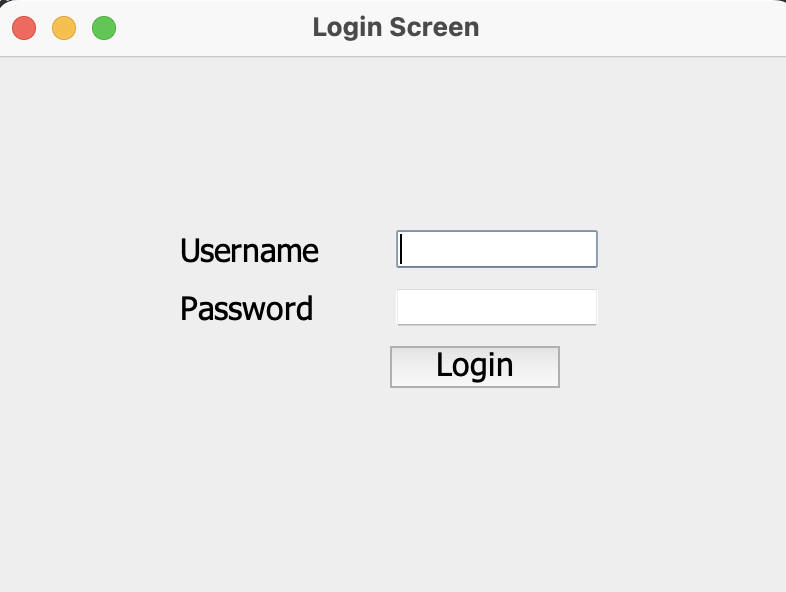
\includegraphics[width=0.5\textwidth]{assets/login-screen.png}
	\caption{Tampilan layar login}
	\label{fig:login-screen}
\end{figure}

\begin{figure}[h!]
	\centering
	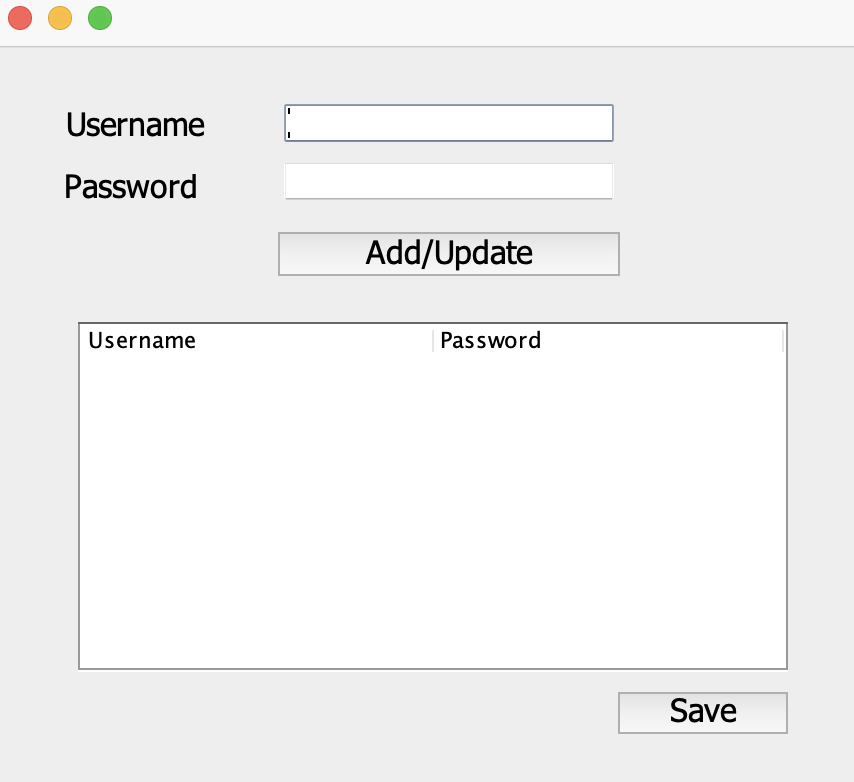
\includegraphics[width=0.5\textwidth]{assets/add-user-form.png}
	\caption{Tampilan formulir tambah pengguna}
	\label{fig:add-user-form}
\end{figure}

\textbf{Keterangan Gambar:} 
\begin{itemize}
	\item Gambar \ref{fig:login-screen}: Menampilkan tampilan GUI untuk login.
	\item Gambar \ref{fig:add-user-form}: Menampilkan tampilan GUI untuk menambah pengguna.
\end{itemize}



\section{Latihan dan Contoh Kode: Aplikasi Manajemen Buku}

\subsection{1. Kelas Book}

\begin{lstlisting}[style=JavaStyle]
	package edu.pradita.p10;
	
	public class Book {
		
		private String title;
		private String author;
		private int year;
		
		public Book(String title, String author, int year) {
			this.title = title;
			this.author = author;
			this.year = year;
		}
		
		public String getTitle() {
			return title;
		}
		
		public void setTitle(String title) {
			this.title = title;
		}
		
		public String getAuthor() {
			return author;
		}
		
		public void setAuthor(String author) {
			this.author = author;
		}
		
		public int getYear() {
			return year;
		}
		
		public void setYear(int year) {
			this.year = year;
		}
	}
\end{lstlisting}

\subsection{2. Kelas Data untuk Buku}

\begin{lstlisting}[style=JavaStyle]
	package edu.pradita.p10;
	
	import java.io.BufferedReader;
	import java.io.BufferedWriter;
	import java.io.File;
	import java.io.FileReader;
	import java.io.FileWriter;
	import java.io.IOException;
	import java.util.ArrayList;
	import java.util.List;
	
	public class Data {
		
		private static List<Book> books = new ArrayList<>();
		
		public static List<Book> getBooks() {
			return books;
		}
		
		public static List<Book> saveBooks(List<Book> books) {
			try {
				Data.books.clear();
				Data.books.addAll(books);
				
				File file = new File("books.csv");
				FileWriter fw = new FileWriter(file);
				BufferedWriter bw = new BufferedWriter(fw);
				
				for (Book book : Data.books) {
					bw.write(book.getTitle() + "," + book.getAuthor() + "," + book.getYear() + System.lineSeparator());
				}
				
				bw.close();
			} catch (IOException e) {
				e.printStackTrace();
			}
			
			return books;
		}
		
		public static List<Book> loadBooks() {
			try {
				File file = new File("books.csv");
				FileReader fr = new FileReader(file);
				BufferedReader br = new BufferedReader(fr);
				
				String line = br.readLine();
				while (line != null) {
					String[] lineArray = line.split(",");
					books.add(new Book(lineArray[0].trim(), lineArray[1].trim(), Integer.parseInt(lineArray[2].trim())));
					line = br.readLine();
				}
				br.close();
			} catch (IOException e) {
				e.printStackTrace();
			}
			
			return books;
		}
	}
\end{lstlisting}

\subsection{3. Kelas Formulir Buku}

\begin{lstlisting}[style=JavaStyle]
package edu.pradita.p10;

import java.awt.EventQueue;
import java.awt.Font;
import java.awt.GraphicsEnvironment;
import java.awt.event.ActionEvent;
import java.awt.event.ActionListener;
import java.util.ArrayList;
import java.util.List;

import javax.swing.JButton;
import javax.swing.JFrame;
import javax.swing.JLabel;
import javax.swing.JPanel;
import javax.swing.JScrollPane;
import javax.swing.JTable;
import javax.swing.JTextField;
import javax.swing.ListSelectionModel;
import javax.swing.border.EmptyBorder;
import javax.swing.event.ListSelectionEvent;
import javax.swing.event.ListSelectionListener;
import javax.swing.table.DefaultTableModel;

public class BookForm extends JFrame {
	
	/**
	* 
	*/
	private static final long serialVersionUID = 1L;
	private JPanel contentPane;
	private JTextField txtTitle;
	private JTable booksTable;
	private JTextField txtAuthor;
	private JTextField txtYear;
	private JButton btnSave;
	
	public static void main(String[] args) {
		EventQueue.invokeLater(new Runnable() {
			public void run() {
				try {
					BookForm frame = new BookForm();
					frame.setVisible(true);
				} catch (Exception e) {
					e.printStackTrace();
				}
			}
		});
	}
	
	public BookForm() {
		contentPane = new JPanel();
		contentPane.setBorder(new EmptyBorder(5, 5, 5, 5));
		setContentPane(contentPane);
		contentPane.setLayout(null);
		
		JLabel lblTitle = new JLabel("Title");
		lblTitle.setFont(new Font("Tahoma", Font.PLAIN, 16));
		lblTitle.setBounds(37, 33, 96, 13);
		contentPane.add(lblTitle);
		
		txtTitle = new JTextField();
		txtTitle.setFont(new Font("Tahoma", Font.PLAIN, 16));
		txtTitle.setBounds(143, 29, 171, 19);
		contentPane.add(txtTitle);
		txtTitle.setColumns(10);
		
		JLabel lblAuthor = new JLabel("Author");
		lblAuthor.setFont(new Font("Tahoma", Font.PLAIN, 16));
		lblAuthor.setBounds(36, 64, 75, 13);
		contentPane.add(lblAuthor);
		
		txtAuthor = new JTextField();
		txtAuthor.setFont(new Font("Tahoma", Font.PLAIN, 16));
		txtAuthor.setBounds(143, 60, 171, 19);
		contentPane.add(txtAuthor);
		txtAuthor.setColumns(10);
		
		JLabel lblYear = new JLabel("Year");
		lblYear.setFont(new Font("Tahoma", Font.PLAIN, 16));
		lblYear.setBounds(36, 95, 75, 13);
		contentPane.add(lblYear);
		
		txtYear = new JTextField();
		txtYear.setFont(new Font("Tahoma", Font.PLAIN, 16));
		txtYear.setBounds(143, 90, 171, 19);
		contentPane.add(txtYear);
		txtYear.setColumns(10);
		
		JButton btnAddUpdate = new JButton("Add/Update");
		btnAddUpdate.addActionListener(new ActionListener() {
			public void actionPerformed(ActionEvent e) {
				String title = txtTitle.getText().trim();
				String author = txtAuthor.getText().trim();
				int year = Integer.parseInt(txtYear.getText().trim());
				int rowCount = booksTable.getRowCount();
				DefaultTableModel table = (DefaultTableModel) booksTable.getModel();
				
				for (int i = 0; i <= table.getRowCount() - 1; i++) {
					if (title.equals(table.getValueAt(i, 0))) {
						table.setValueAt(author, i, 1);
						table.setValueAt(year, i, 2);
						return;
					}
				}
				table.insertRow(rowCount, new Object[] { title, author, year });
			}
		});
		btnAddUpdate.setFont(new Font("Tahoma", Font.PLAIN, 16));
		btnAddUpdate.setBounds(143, 123, 171, 22);
		contentPane.add(btnAddUpdate);
		
		JScrollPane scrollPane = new JScrollPane();
		scrollPane.setBounds(43, 158, 355, 175);
		contentPane.add(scrollPane);
		
		Object[][] data = new Object[Data.getBooks().size()][3];
		for (int i = 0; i < Data.getBooks().size(); i++) {
			Book book = Data.getBooks().get(i);
			data[i][0] = book.getTitle();
			data[i][1] = book.getAuthor();
			data[i][2] = book.getYear();
		}
		
		booksTable = new JTable();
		booksTable.setModel(new DefaultTableModel(data, new String[] { "Title", "Author", "Year" }) {
			/**
			* 
			*/
			private static final long serialVersionUID = 1L;
			Class[] columnTypes = new Class[] { String.class, String.class, Integer.class };
			
			public Class getColumnClass(int columnIndex) {
				return columnTypes[columnIndex];
			}
			
			boolean[] columnEditables = new boolean[] { false, false, false };
			
			public boolean isCellEditable(int row, int column) {
				return columnEditables[column];
			}
		});
		scrollPane.setViewportView(booksTable);
		booksTable.setSelectionMode(ListSelectionModel.SINGLE_SELECTION);
		booksTable.setFont(new Font("Tahoma", Font.PLAIN, 16));
		booksTable.getSelectionModel().addListSelectionListener(new ListSelectionListener() {
			@Override
			public void valueChanged(ListSelectionEvent e) {
				String title = booksTable.getValueAt(booksTable.getSelectedRow(), 0).toString();
				String author = booksTable.getValueAt(booksTable.getSelectedRow(), 1).toString();
				int year = (int) booksTable.getValueAt(booksTable.getSelectedRow(), 2);
				txtTitle.setText(title);
				txtAuthor.setText(author);
				txtYear.setText(String.valueOf(year));
			}
		});
		
		btnSave = new JButton("Save");
		btnSave.addActionListener(new ActionListener() {
			public void actionPerformed(ActionEvent e) {
				List<Book> books = new ArrayList<>();
				for (int i = 0; i < booksTable.getModel().getRowCount(); i++) {
					String title = booksTable.getValueAt(i, 0).toString(); 
					String author = booksTable.getValueAt(i, 1).toString(); 
					int year = Integer.parseInt(booksTable.getValueAt(i, 2).toString());
					books.add(new Book(title, author, year));
				}
				
				Data.saveBooks(books);
			}
		});
		btnSave.setFont(new Font("Tahoma", Font.PLAIN, 16));
		btnSave.setBounds(143, 346, 171, 22);
		contentPane.add(btnSave);
		
		this.setDefaultCloseOperation(JFrame.EXIT_ON_CLOSE);
		this.setBounds(centerX(500), centerY(450), 500, 450);
		this.setVisible(true);
	}
	
	private int centerX(int frameWidth) {
		return GraphicsEnvironment.getLocalGraphicsEnvironment().getCenterPoint().x - (frameWidth / 2);
	}
	
	private int centerY(int frameHeight) {
		return GraphicsEnvironment.getLocalGraphicsEnvironment().getCenterPoint().y - (frameHeight / 2);
	}
}
\end{lstlisting}

\begin{figure}[h!]
	\centering
	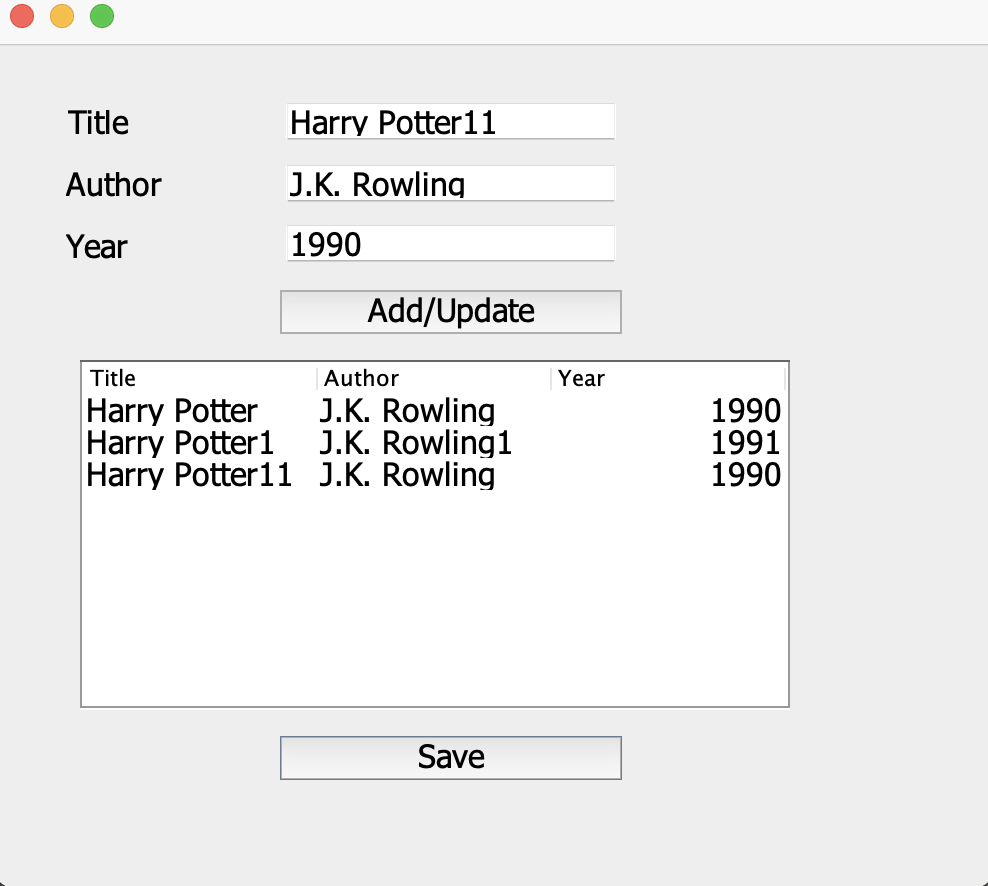
\includegraphics[width=0.5\textwidth]{assets/book-form.png}
	\caption{Tampilan layar book form}
\end{figure}



\section{Soal}

\subsection*{Soal 1: Aplikasi Manajemen Karyawan}

\textbf{Konteks dan Kasus:} \\
Anda diminta untuk membuat aplikasi manajemen karyawan di sebuah perusahaan. Setiap karyawan memiliki nama, jabatan, dan gaji. Aplikasi ini memungkinkan pengguna untuk menambahkan karyawan baru, mengedit informasi karyawan yang sudah ada, dan menyimpan data karyawan ke dalam file CSV.

\textbf{Tugas:}
\begin{enumerate}
	\item Buat kelas \texttt{Employee} yang memiliki atribut \texttt{name}, \texttt{position}, dan \texttt{salary}.
	\item Implementasikan kelas \texttt{EmployeeData} untuk memanage data karyawan termasuk menyimpan dan memuat data ke/dari file CSV.
	\item Implementasikan GUI untuk mengelola data karyawan dalam aplikasi.
	\item Tambahkan fitur untuk menghitung total gaji semua karyawan dan menampilkannya di dalam GUI.
\end{enumerate}

\subsection*{Soal 2: Aplikasi Pengelolaan Inventori Barang}

\textbf{Konteks dan Kasus:} \\
Sebuah toko retail ingin membuat aplikasi untuk mengelola inventori barang. Setiap barang memiliki nama, kategori, dan jumlah stok. Aplikasi ini memungkinkan pengguna untuk menambahkan barang baru, mengedit informasi barang yang ada, dan menyimpan data barang ke dalam file CSV.

\textbf{Tugas:}
\begin{enumerate}
	\item Buat kelas \texttt{Product} yang memiliki atribut \texttt{name}, \texttt{category}, dan \texttt{quantity}.
	\item Implementasikan kelas \texttt{InventoryData} untuk mengelola data barang termasuk menyimpan dan memuat data ke/dari file CSV.
	\item Implementasikan GUI untuk mengelola data barang dalam aplikasi.
	\item Tambahkan fitur untuk memantau stok barang, dengan memberikan peringatan jika stok barang tertentu kurang dari jumlah minimum yang ditentukan.
\end{enumerate}